\documentclass[12pt]{article}
\usepackage{amsmath, amssymb, amsthm}
\usepackage{import}
\usepackage{pdfpages}
\usepackage{transparent}
\usepackage{xcolor}
\usepackage{graphicx}
\usepackage[framed, numbered]{matlab-prettifier}

\usepackage{fancyhdr}

\fancyhf{}
\pagestyle{fancy}
\lhead{Carrera}
\rhead{\thepage}

\setlength\parindent{0pt}
\numberwithin{equation}{section}

%\usepackage{titlesec}
%\titleformat{\section}
%{\normalfont\Large\bfseries}{Exercise~\thesection}{1em}{}

\newcommand{\incfig}[2][1]{%
  \def\svgwidth{#1\columnwidth}
  \import{./figures/}{#2.pdf_tex}
}

\newcommand{\RE}{\mathrm{Re}}
\newcommand{\IM}{\mathrm{Im}}

\newcommand\ddfrac[2]{\frac{\displaystyle #1}{\displaystyle #2}}
\newcommand\eval{\bigg\rvert}

\pdfsuppresswarningpagegroup=1

\author{Adam Carrera}
\date{February 1, 2021}
\title{MECH 4110 - Pre-lab \#2}

\begin{document}
  \maketitle

  \section{Linearization}

  Linearize Prelab 2 Equation (1.3.16) about a general operating point $ (\bar h_1, \, \bar v_p). $ First, write Prelab 2 Equation (1.3.16) in the form of $ \dot h_1 = f(h_1, v_p). $

  \begin{equation}
    \dot h_1 = \frac{K_p}{A_c} (v_p - v_p^{min}) - \frac{C_d A_o}{A_c}\sqrt{2gh_1}
  \end{equation}

  We can linearize the above equation with a Taylor Series Expansion. Evaluate the derivatives at the operating point $ (\bar h_1, \, \bar v_p). $

  \begin{equation}
    \Delta \dot h_1 = \frac{df}{dh_1} \Delta h_1 + \frac{df}{dv_p} \Delta v_p
  \end{equation}

  where,

  \begin{align}
    \frac{df}{dh_1}\eval_{\bar h_1, \bar v_p} &= -\frac{C_d A_o g}{A_c\sqrt{2g\bar h_1}} \\
    \frac{df}{dv_p}\eval_{\bar h_1, \, \bar v_p} &= \frac{K_p}{A_c}
  \end{align}

  Therefore, the linearized system is,

  \begin{equation}\label{eq:eq1}
    \Delta \dot h = -\frac{C_d A_o g}{A_c\sqrt{2g\bar h_1}} \Delta h_1 + \frac{K_p}{A_c} \Delta v_p
  \end{equation}

  \newpage

  \section{Open Loop Transfer Function}

  Using Equation (\ref{eq:eq1}) we can find the open loop transfer function. We have,

  \begin{equation}
    \dot y + \frac{C_d A_o g}{A_c\sqrt{2g\bar y}} y = \frac{K_p}{A_c} u
  \end{equation}

  \begin{equation}
    A_c \sqrt{2g \bar y} \dot y + C_d A_o g y = K_p \sqrt{2g\bar y} u
  \end{equation}

  \begin{equation}
    \frac{A_c\sqrt{2g\bar y}}{C_d A_o g} \dot y + y = \frac{K_p}{C_d A_o g}\sqrt{2g \bar y} u
  \end{equation}

  Take the laplace transform of both sides

  \begin{equation}
    Y(s) \left( \frac{A_c\sqrt{2g\bar y}}{C_d A_o g} + 1 \right) = \frac{K_p}{C_d A_o g}\sqrt{2g \bar y} U(s)
  \end{equation}

  Therefore,

  \begin{equation}\label{eq:eq2}
    G(s) = \frac{Y(s)}{U(s)} = \ddfrac{\frac{K_p}{C_d A_o g}\sqrt{2g \bar y}}{\frac{A_c\sqrt{2g\bar y}}{C_d A_o g} + 1}
  \end{equation}

  Compare Equation (\ref{eq:eq2}) to Prelab 2 Equation (1.3.6). Clearly,

  \begin{equation}
    \tau = \frac{A_c\sqrt{2g\bar y}}{C_d A_o g}
  \end{equation}

  \begin{equation}
    K_{DC} = \frac{K_p}{C_d A_o g}\sqrt{2g \bar y}
  \end{equation}

  \newpage

  \section{Closed Loop Transfer Function}

  Let $ G(s) = \frac{K_{DC}}{\tau s + 1}, \, C(s) = \frac{k_ps + k_i}{s}. $ $ G $ is the open loop transfer function derived in section 2, $ C $ is a PI controller. We can find the closed loop transfer function with

  \begin{equation}
    \frac{Y}{R} = \frac{GC}{1 + GC}
  \end{equation}

  Using MATLAB to compute the expression, we get

  \begin{equation}\label{eq:eq3}
    \frac{Y}{R} = \frac{K_{DC}(k_i + k_ps)}{\tau s ^2 + (K_{DC}k_p + 1)s + K_{DC}k_i}
  \end{equation}

  \lstinputlisting[style=Matlab-editor, caption = {Determination of Closed Loop Transfer Function}]{../MATLAB Files/prelab2.m}

  \begin{figure}
    \centering
    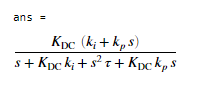
\includegraphics[width=0.5\textwidth]{figures/answer}
    \caption{Output of Listing 1}
    \label{fig:fig1}
  \end{figure}

  \newpage

  \section{Determination of $ k_i, k_p. $}

  Compare the denominator of Equation (\ref{eq:eq3}) to Prelab 2 Equation (1.3.10).

  We find that,

  \begin{equation}
    \omega_n^2 = \frac{K_{DC}k_i}{\tau} \Rightarrow k_i = \frac{\omega_n^2}{K_{DC}}\tau
  \end{equation}

  \begin{equation}
    2\zeta\omega_n = \frac{K_{DC}k_p + 1}{\tau} \Rightarrow k_p = \frac{2\tau\zeta\omega_n - 1}{K_DC}
  \end{equation}






\end{document}
